\documentclass{article}
\usepackage[utf8]{inputenc}
\usepackage{minted}
\usepackage{natbib}
\usepackage[spanish]{babel}
\usepackage{graphicx}
\usepackage{pgfgantt}
\usepackage{pdflscape}
\usepackage{afterpage}
\graphicspath{ {imagenes/} }
\usepackage{eurosym}
\usepackage{placeins}

\usepackage{geometry}
 \geometry{
 a4paper,
 total={170mm,257mm},
 left=35mm,
 right=25mm,
 top=20mm,
 }


\renewcommand{\theenumii}{\theenumi.\arabic{enumii}.}  % 2nd level of enumerate with numbers
\renewcommand{\labelenumii}{\theenumii} % 2ndd level of enumerate with numbers
\author{Adrián Gil Moral }

\newcommand{\cool}[1] {
    {\texttt{#1}}
}

\begin{document}
\section{Planificación del proyecto}
\paragraph{}
En esta sección se abordará tanto la planificación temporal del proyecto como el coste económico estimado para el desarrollo de este proyecto.

\subsection{Planificación temporal}
\paragraph{}
En el siguiente gráfico de Gantt se puede ver cómo se ha distribuído el tiempo necesario para desarrollar este proyecto. Tras este, se desglosa de manera resumida en qué ha consistido el trabajo desarrollado en cada una de las etapas expuestas en este diagrama.

\begin{landscape}
\thispagestyle{empty}
\begin{figure}[H]
    
    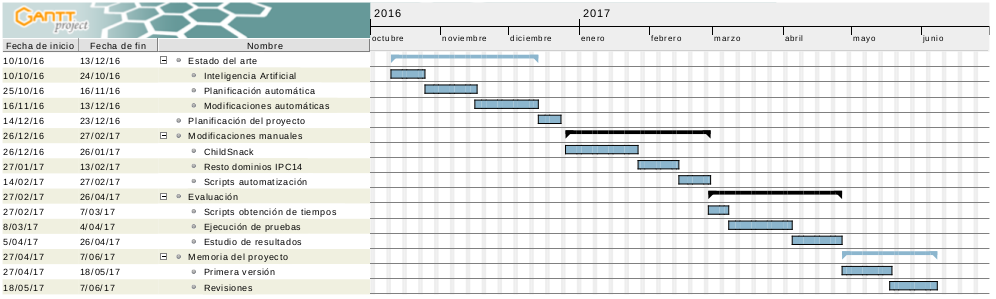
\includegraphics[width=20cm, height=11cm]{diagramaGantt}
    \caption{Diagrama de Gantt del proyecto}
\end{figure}
\end{landscape}

\begin{itemize}
    \item Estado del arte: el primer paso que se ha dado ha sido investigar sobre lo que se ha hecho en el campo de estudio en el que se va a trabajar. En esta fase la mayor parte de la sección de la memoria que lleva este mismo título ha sido redactada mientras que en otra se ha dejado un pequeño esquema minimalista sobre la materia que sirviera simplemente para saber lo que se ha hecho en este campo para tenerlo en cuenta al implementar la solución. Estas partes que no han sido redactadas para poder ser incluidas directamente en este proyecto han sido luego desarrolladas en la fase de redacción de la memoria del proyecto. Como se puede ver el en órden cronológico de las subtareas, se ha seguido un órden que implique pasar de lo más genérico a cada vez lo más concreto en relación con el tema de este trabajo.
    
    \begin{itemize}
        \item Inteligencia artificial: como ya se tenían ciertas nociones sobre este área, la búsqueda ha ido encaminada a la parte histórica de la inteligencia artificial y sus posibles diferentes secciones para así incluirlo en la memoria más que para adquirir un nuevo conocimiento que realmente se aplicase en la solución propuesta.
        \item Planificación automática: antes de empezar este proyecto, ya se había trabajado con planificadores automáticos de PDDL. Sin embargo, en estos trabajos previos el planificador operaba como una caja negra. Por tanto, esta sección ha sido muy necesaria para intentar entender el funcionamiento detrás de lo que antes era una caja negra para así poder interpretar de manera más acertada los resultados obtenidos tras la planificación automática.
        \item Modificaciones automáticas: como se ha reflejado en la memoria, existe trabajo previo de otros investigadores que han realizado programas para automatizar la representación de dominios en PDDL, siendo algunos de ellos independientes o dependientes de dominio. El código de las modificaciones independientes de dominio más prometedoras que se han conseguido ejecutar con éxito han sido incluidas en la sección de pruebas de esta memoria.
    \end{itemize}
    
    \item Modificaciones manuales: al estudiar un dominio, es posible encontrar la forma de modificar la representación del mismo para reducir la búsqueda del planificador para así obtener soluciones óptimas y completas en un menor tiempo de búsqueda respecto a la versión original. En esta sección se ha hecho este estudio y sus modificaciones con distintos dominios.
    
    \begin{itemize}
        \item ChildSnack: este es el principal dominio con el que se han realizado todas las pruebas y por ello se ha dedicado más tiempo a este dominio que a la suma del tiempo dedicado a todos los demás dominios analizados.
        \item Resto dominios IPC14: para intentar generalizar algunas de las conclusiones de este proyecto, se han analizado otros dominios de la misma edición en la que se presentó el dominio ChildSnack a la IPC.
        \item Scripts automatización: algunas de las modificaciones realizadas a mano en el dominio de ChildSnack se han automatizado mediante scripts para así poder transformar de manera automática los problemas del dominio original.
    \end{itemize}
    
    \item Evaluación: en esta fase se han evaluado las distitnas versiones de ChildSnack con varios planificadores automáticos.
    
    \begin{itemize}
        \item Scripts de obtención de tiempos: se ha creado un script que dado un dominio, una carpeta de problemas y uno de los planificadores para los que está diseñado el dominio, devuelve un archivo de texto plano con todos los tiempos de ejecución, la calidad de la solución así como guarda el plan en caso de haber encontrado la solución al problema.
        \item Ejecución de pruebas: esta fase ha consistido en la ejecución del script con los distintos parámetros de entrada y comprobación de una muestra de los resultados para verificar que no ha habido ningún problema en la ejecución.
        \item Estudio de resultados: una vez se ha verificado que los datos obtenidos son correcto, es necesario interpretarlos ya que la comparación de los mismos determinará su exposición en la memoria.
    \end{itemize}
    
    \item Memoria del proyecto: una vez se han realizado todas las pruebas, se han documentado todo el proceso seguido así como se ha dejado por escrito la interpretación de los resultados obtenidos y las líneas futuras de investigación. Antes de empezar esta fase, únicamente estaba redactada alguna sección del estado del arte de la memoria que ha sido revisada en esta fase.
    
    
    \begin{itemize}
        \item Primera versión: se ha realizado una primera versión de todo el proyecto para entregar a la profesora y que a partir de esta realizase las anotaciones correspondientes para posteriores versiones.
        \item Revisiones: las posteriores versiones de la memoria han sido trabajadas tanto a partir de la totalidad de la memoria en distintas revisiones como mediante revisiones concretas de cada una de las secciones de la memoria.
    \end{itemize}
\end{itemize}

\paragraph{}
Resumiendo, entre la fecha de inicio y la fecha de finalización del proyecto han trascurrido \\ $341 d\´ias = \ceil{\frac{241 d\´ias}{7 d\´ias/semana}} = 35 semanas$. Si estimamos una media de $13 horas/semana$ a este proyecto, el total de horas dedicadas al proyecto por el alumno es de \textbf{$35 semanas * 13 horas/semana=455 horas$}. Estas horas incluyen las horas invertidas en tutorías especificadas a continuación pero no las horas de ejecución de las pruebas automatizadas.

\paragraph{}
La planificación ha estado fuertemente influida por las diversas reuniones entre el alumno y la tutora. A continuación se incluye esta información que servirá tanto para plasmar la planificación de este proyecto como para la estimación ulterior de la estimación de gasto en recursos humanos para la realización de este proyecto.
\begin{enumerate}
    \item 21 de septiembre de 2016.
    \item 10 de octubre de 2016.
    \item 25 de octubre de 2016
    \item 23 de noviembre de 2016
    \item 14 de diciembre de 2016
    \item 20 de febrero de 2017
    \item 14 de marzo de 2017
    \item 4 de abril de 2017
    \item 27 de abril de 2017
    \item 24 de mayo de 2017
    \item 29 de mayo de 2017 
\end{enumerate}

\paragraph{}
La duración media de estas reuniones ha sido de en torno a 105 minutos, por lo tanto se estima el número de horas invertidas en estas tutorías en \\ $\ceil{1.75 horas/tutor\´ia * 11 tutor\´ias} = 20 horas$. Se estima a su vez que para 6 de estas tutorías ha sido necesario el trabajo previo de $2 horas$ por parte de la tutora, sumado a $8 horas$ dedicadas para las distintas revisiones de la memoria, lo que hace un total de \\ $20 + 6 * 2 + 8 = 40 horas$. Esta cifra será más adelante utilizada para estimar el coste económico de recursos humanos.

\section{Estimación de costes económicos}

\paragraph{}
Esta sección versa sobre el coste económico de la realización de este proyecto en caso de haberse tenido que realizar sin contar con ningún material previo (como pueda ser un ordenador de sobremesa) ni con la idiosincracia de pago de personal académico en la universidad. Es decir, la estimación de costes que se muestra toma como marco de referencia la empresa privada así como la separación de trabajadores según las áreas de trabajo que se pueden encontrar en empresas tecnológicas grandes. Según las recomendaciones de Bruselas acatadas por España en el año 2013, se considera una empresa grande a partir de 250 trabajadores\cite{empresaGrande}.

\subsection{Recursos materiales}
\begin{table}[H]
\centering
\caption{Recursos materiales}
\label{my-label}
\begin{tabular}{|c|c|c|c|c|c|}
\hline
\textbf{Concepto}      & \textbf{Unidades} & \textbf{Coste/u} & \textbf{Total} & \textbf{Amortización/mes} & \textbf{Amortizado (8 meses)} \\ \hline
Ordenador de sobremesa & 1                           & 649\euro                     & 649\euro                  & 2,08\%                                      & 107,99\euro                                       \\ \hline
Pantalla del ordenador & 1                           & 79\euro                      & 79\euro                   & 2,08\%                                      & 13,15\euro                                        \\ \hline
Router                 & 1                           & 22\euro                      & 22\euro                   & 2,08\%                                      & 3,66\euro                                         \\ \hline
\textbf{Total}         & -                           & -                       & 750\euro                  & -                                           & 124,8\euro                                        \\ \hline
\end{tabular}
\end{table}

\paragraph{}
Antes de poder estimar el coste de materiales fungibles, es necesario calcular las horas de electricidad que han sido necesarias para que el ordenador estuviese encendido con el fin de realizar este proyecto. Para ello hay que añadir a las horas de trabajo del alumno frente al ordenador el número de horas de ejecución de las pruebas.

\paragraph{}
Teniendo en cuenta que todos los artículos y libros citados en la bibliografía han sido consultados a través del ordenador, las únicas horas del proyecto que no se ha utilizado este dispositivo es cuando el alumno se encontraba en una tutoría del proyecto. Por tanto, el número de horas en las que se ha hecho uso del ordenador sin contar las horas de pruebas es de $455 horas - 20 horas = 435 horas$.

\paragraph{}
Respecto a las horas necesarias para ejecutar las diversas pruebas, primero hay que tomar en cuenta que aunque en la versión que se ha presentado de este trabajo existan 12 dominios distintos de Childsnack, antes de cribar las versiones menos prometedoras el número de estos dominios era de 16 dominios. Estos 4 dominios descartados eran de baja calidad por lo que para esta estimación se asumirá que únicamente resolvían 2 de los 20 problemas en 30 segundos cada uno, por lo que para simplificar la estimación al ser un tiempo nimio esta cantidad no será tomada en cuenta. Teniendo en cuenta que el tiempo límite de búsqueda de los planificadores es de 30 minutos y que dichas pruebas se ejecutaron 2 veces, el tiempo consumido en la prueba de estos 4 dominios descartados es de $4 * (0.5 horas/problema * 18 problemas)/ejecuci\´on * 2 ejecuciones = 72 horas$. Esta cifra corresponde al número de horas de ejecución necesarias por cada planificador utilizado. Como se han utilizado dos planificadores, el número total será: $72 horas/planificador * 2 planificadores = 144 horas$.

\paragraph{}
De la versión final se han conservado los tiempos de ejución para cada planificador, ya que dichos resultados han sido analizados en la sección de evaluación de resultados. Por tanto, teniendo en cuenta que estas pruebas también se han realizado 2 veces, que se han realizado las pruebas con 2 planificadores y tomando la simplificación de descartar el tiempo de las ejecuciones en las que se ha resuelto el problema y añadir un total de $3 horas/ejecuci\´on * 2 ejecuciones = 6 horas$ horas que es un tiempo superior al de la suma del tiempo necesario para la obtención de todas las soluciones para todos los problemas de todas las versiones, obtenemos: \\

$97 problemas no resueltos MFF/iteraci\´on * 2 iteraciones + $ \\
$42 problemas no resueltos LPG-td/iteraci\´on * 2 iteraciones$ \\
$= 278 problemas no resueltos * 0.5horas/problema no resuelto = 139 horas$

Por tanto, el número de horas de electricidad necesarias para alimentar el ordenador durante este proyecto será de $435 + 144 + 6 + 139 horas = 724 horas$ de luz necesarias.

\paragraph{}
El coste de materiales fungibles es el siguiente:

\begin{table}[H]
\centering
\caption{Coste de materiales fungibles}
\label{my-label}
\begin{tabular}{|l|l|l|l|}
\hline
\textbf{Concepto}                         & \textbf{Unidades}      & \textbf{Coste/u}          & \textbf{Total}              \\ \hline
Material para escribir                    & 1                      & 9                         & 9                           \\ \hline
Hora de electricidad                      & 724                    & 0.1358\euro/KWhora        & 98,32                       \\ \hline
\multicolumn{1}{|c|}{Conexión a internet} & \multicolumn{1}{c|}{8} & \multicolumn{1}{c|}{19,2} & \multicolumn{1}{c|}{153,6}  \\ \hline
\multicolumn{1}{|c|}{\textbf{Total}}      & \multicolumn{1}{c|}{-} & \multicolumn{1}{c|}{-}    & \multicolumn{1}{c|}{260,92} \\ \hline
\end{tabular}
\end{table}

\paragraph{}
Por tanto, la estimación de gastos materiales totales para este proyecto es de \\ $124,8€ + 260,92€ = 385,72€$. A esta cantidad habría que añadirle la cantidad no amortizada en los 8 meses de duración de proyecto que sin embargo sin necesarios para comprar el material para desarrollar este proyecto. Es decir, sería necesario disponer a su vez de $750€ - 124,8€  = 625,2€$ de inversión inicial.

\paragraph{}
Se quiere volver a insistir en que estos datos son estimatorios y simplificados. Otros gastos como el gasto de luz para la iluminación o la calefación durante el invierno han sido descartados.

\subsection{Recursos humanos}
\paragraph{}
Para este proyecto se pueden dividir las tareas realizadas en tantos empleados como la imaginación pueda dar de sí. Estas distintas versiones podrían luego ser estimadas y con ello extraer el coste económico correspondiente a la remuneración de estos trabajadores. Sin embargo, para que esta estimación sea más realista, se va a asumir como coste de desarrollo de este proyecto la composición real que ha tenido (una profesora y un alumno) pero cambiando dichos roles por su equivalente en la empresa privada (como puede ser el project manager y el programador raso).

\begin{table}[H]
\centering
\caption{Coste recursos humanos}
\label{my-label}
\begin{tabular}{|c|c|c|c|}
\hline
\textbf{Posición} & \textbf{Coste/hora} & \textbf{Horas} & \textbf{Total} \\ \hline
Project manager   & 35                  & 40             & 1400           \\ \hline
Programador       & 25                  & 455            & 11375          \\ \hline
Total             & -                   & -              & 12775          \\ \hline
\end{tabular}
\end{table}

\subsection{Coste total}

\paragraph{}
El coste total de este proyecto será igual al sumatorio de los costes de los materiales fungibles, físicos, el coste en recursos humanos así como el porcentaje de ganancia y el porcentaje de riesgos, como puede ser que el terminal utilizado deje de estar operativo. Este sumatorio se resume en la tabla que se muestra a continuación.

\begin{table}[H]
\centering
\caption{Coste total del proyecto}
\label{my-label}
\begin{tabular}{|c|c|}
\hline
\textbf{Concepto}  & \textbf{Coste} \\ \hline
Recursos físicos   & 124,8\euro          \\ \hline
Recursos fungibles & 260,92\euro         \\ \hline
Recursos humanos   & 12.775\euro         \\ \hline
Beneficios         & 2.632,14\euro       \\ \hline
Riesgos            & 1974,11\euro        \\ \hline
Total              & \textbf{17766,97\euro}       \\ \hline
\end{tabular}
\end{table}

\end{document}